%!TEX root = ../../../adrien_gomar_phd.tex

As shown above, in a single rotor propeller, the outlet velocity is not axial
yielding a residual tangential velocity $\Delta V_{\theta}$. 
This tangential velocity forms the swirl. 
This is a lost energy that deteriorates the propulsive efficiency. 
To recover this lost energy, a second contra-rotating rotor can be used~\cite{Hager1988}.
We will see in this section through a simple velocity triangle exercise that
the swirl is annulated by the second rotor. This increases the propulsive
efficiency as shown by \citet{Hughes1989} and reported 
in Fig.~\ref{fig:hughes_propulsive_efficiency}.
\begin{figure}[htp]
  \centering
  \includegraphics*[width=0.40\textwidth]{hughes_propulsive_efficiency}
  \caption{Benefit of using a contra-rotating open rotor, from \citet{Hughes1989}.}
  \label{fig:hughes_propulsive_efficiency}
\end{figure}

\subsection{Geometry}
\label{sub:cror_geometry}

Figure~\ref{fig:cror_geometry} depicts the main
geometrical parameters of a CROR.
It is composed of two rotors, the first one is called
the front rotor and the second one is called the rear or aft rotor.
Generally, they do not have the same diameter $D$ and rotation speed
$| \Omega |$. Thus, subscript $f$ and $r$ denotes respectively,
the front and the rear parameter.
As the rotors are contra-rotating, their rotation speed is opposed.
The difference of diameter is called the clipping or cropping
of the blades and is evaluated through the non-dimensional parameter
$\kappa$:
\begin{equation}
    \kappa = \frac{D_f - D_r}{D_f}.
\end{equation}
This clipping is done to avoid the interaction 
with the rear rotor of the tip vortex shed
by the front rotor. In fact, by clipping the rear
rotor, tip vortex of the front rotor is not likely
to hit the rear rotor.
Finally, the spacing between the rotors
is evaluated as the difference between the axial minimum of the
rear blade minus the axial maximum of the front blade. The spacing
is one of the adjustment parameters used to minimize the unsteady
interaction between the rotors to reduce noise. In fact, 
heterogeneities are lessened along with the convection of
the flow field, and these heterogeneities are responsible
of the unsteady interactions.
\begin{figure}[htp]
  \centering
  \includegraphics*[scale=0.3]{cror_geometry.pdf}
  \caption{Contra-rotating open rotor geometrical parameters.}
  \label{fig:cror_geometry}
\end{figure}

Two types of contra-rotating open rotors have emerged, the
puller CROR whose blades are in front of the spinner as 
shown in Fig.~\ref{fig:cror_configurations}. As it
name indicates, this configuration is mounted in front of the
wing. It is particularly interesting as the blades will see
a uniform flow. However, these all suffer from the same incidence as that
of the wing. This can give large in-plane forces compared to pusher
configurations. In fact, the deflection of the flow due to the wing provides
a smaller incidence.
Moreover, the distortion generated
by the CROR will disturb the flow around the wing. As one way to reduce
consumption of airplanes is to have laminar wings, this configuration
is less studied. The second configuration is the pusher
configuration. This is designed to be mounted on a pylon which
interacts with the CROR, but laminar wings might be considered with
this configuration. In this thesis, we will deal with a pusher configuration
in Chapters~\ref{cha:dream_ls_isolated} and
\ref{cha:dream_hs_isolated}.
\begin{figure}[htp]
  \centering
  \subfigure[Puller]{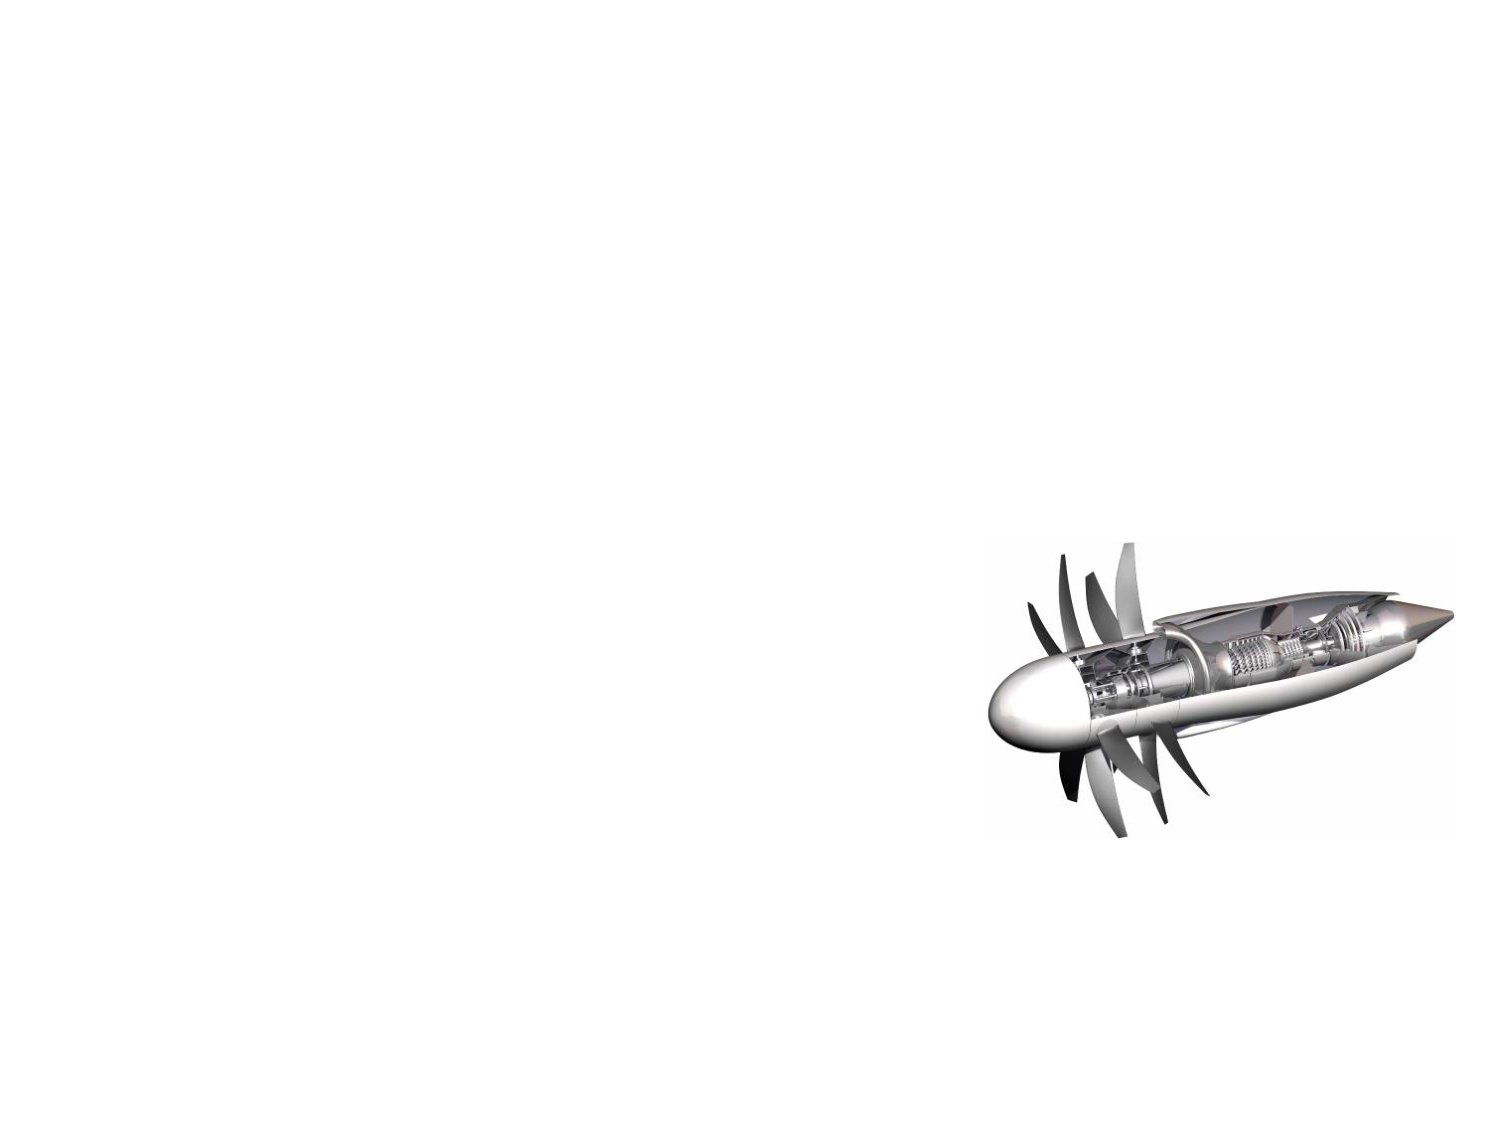
\includegraphics[width=.4\textwidth]{puller.pdf}}
  \subfigure[Pusher]{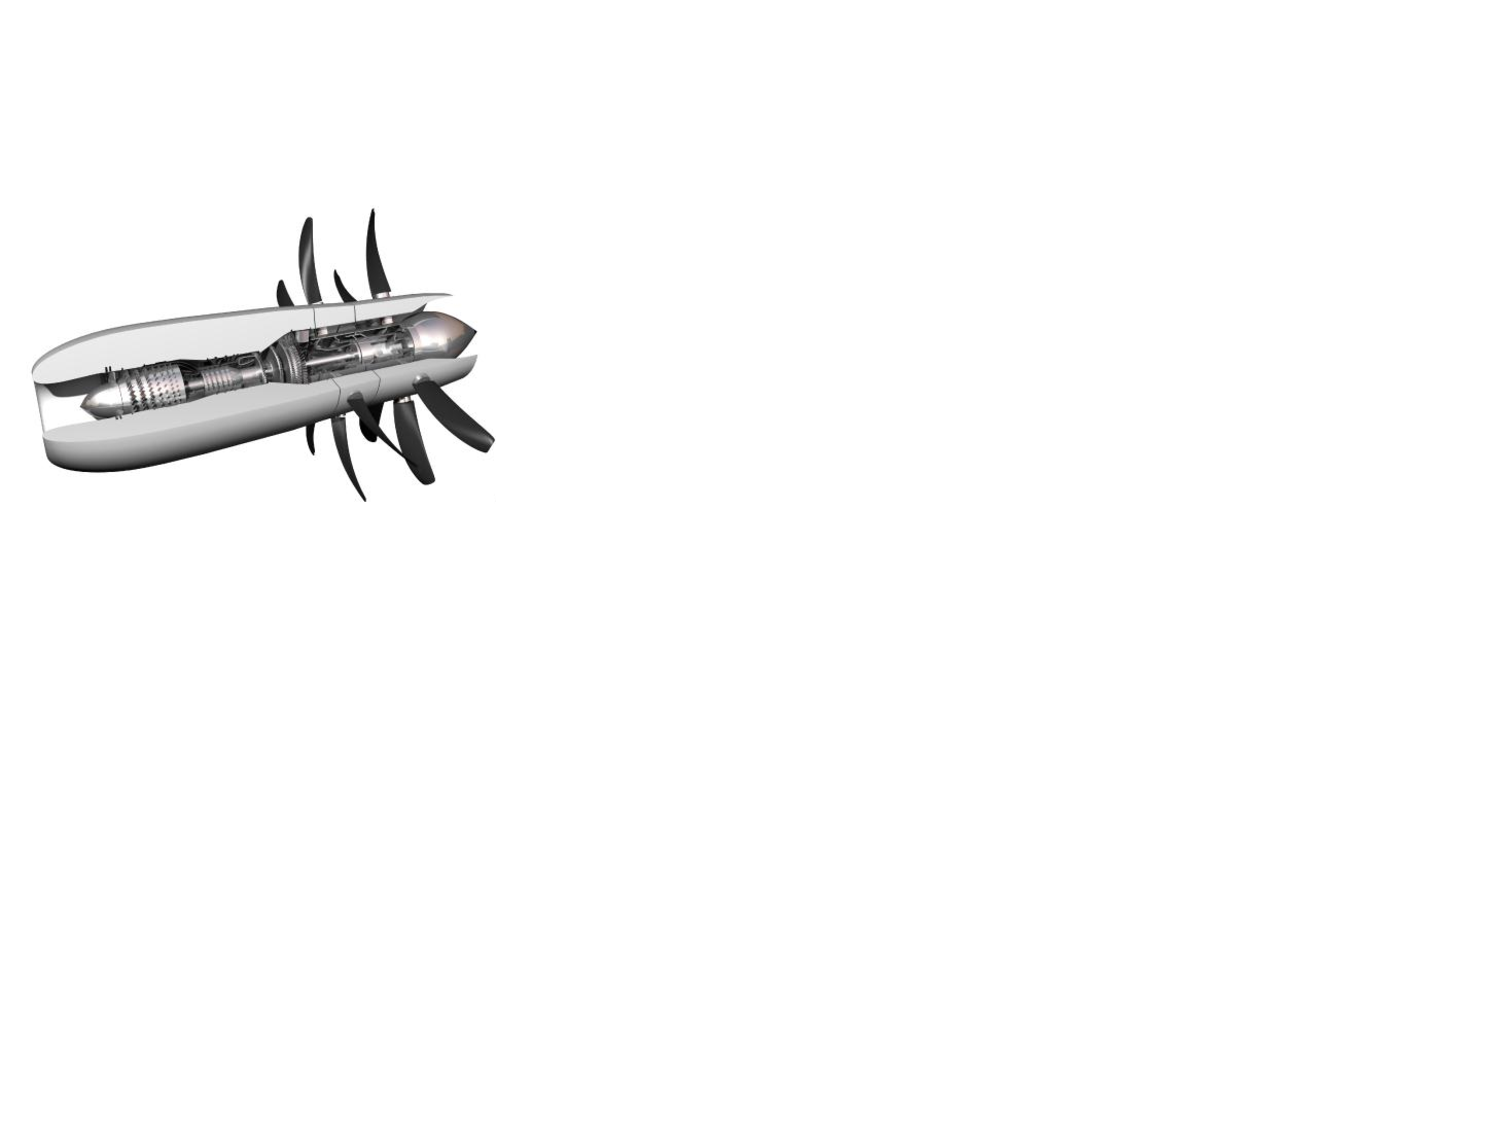
\includegraphics[width=.4\textwidth]{pusher.pdf}}
  \caption{Contra-rotating open rotor configurations, courtesy Rolls-Royce.}
  \label{fig:cror_configurations}
\end{figure}

For pusher CROR, two types of architectures can be thought:
one based on a gearbox and the second
being build around a statorless low-pressure turbine.
\begin{figure}[htp]
  \centering
  \subfigure[Geared design]{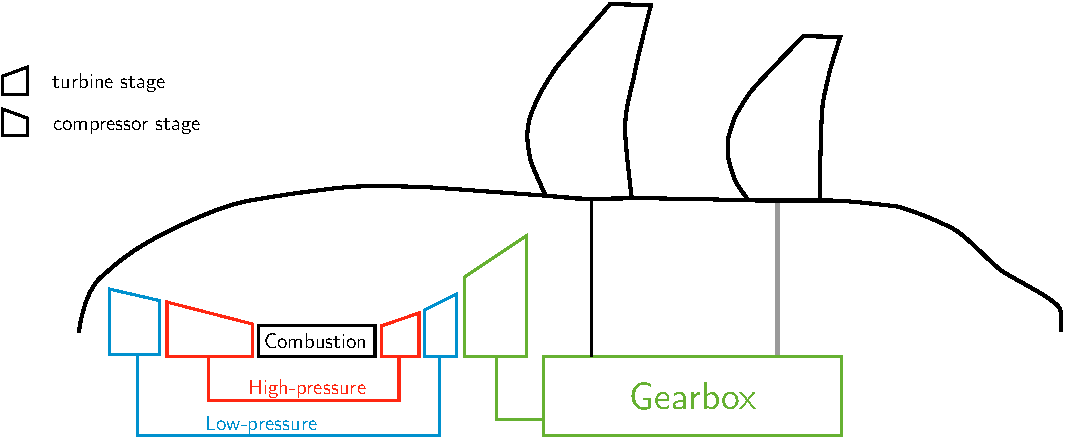
\includegraphics[width=.4\textwidth]{geared_cror.pdf}}
  \subfigure[Statorless low-pressure turbine design]{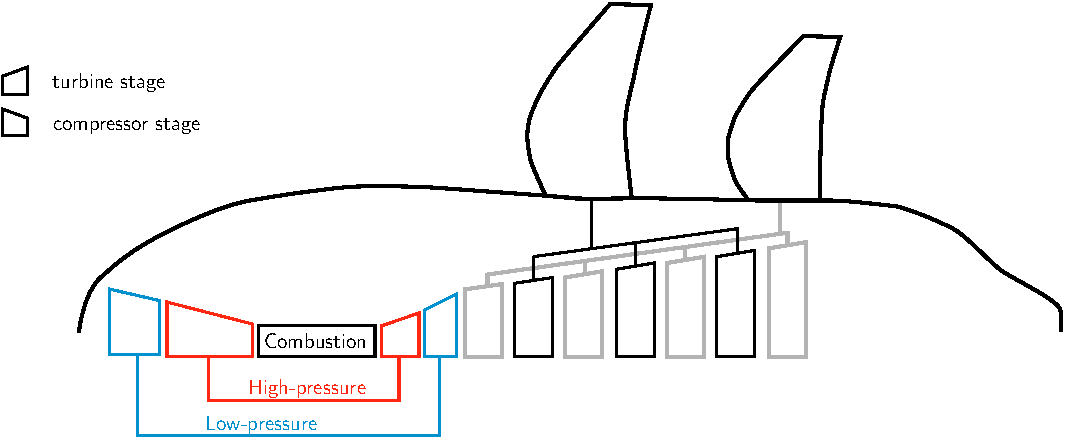
\includegraphics[width=.4\textwidth]{stator_less_cror.pdf}}
  \caption{Contra-rotating open rotor pusher architectures.}
  \label{fig:cror_architectures}
\end{figure}

\subsection{Velocity triangle}
\label{sub:cror_velocity_triangle}
\begin{figure}[htp]
  \centering
  \includegraphics*[scale=0.40]{velocity_triangle_cror.pdf}
  \caption{Velocity triangle applied to a contra-rotating open rotor configuration.}
  \label{fig:velocity_triangle_cror}
\end{figure}
Figure~\ref{fig:velocity_triangle_cror} shows the application
of the velocity triangle to a CROR configuration. The swirl
energy that was lost in the propeller is now used to 
produce more thrust. Thus, a CROR has a better propulsive
efficiency than a propeller, which explains its study as
a greener engine. In the eighties, 
\citet{Strack1981} and \citet{Hager1988} showed that
using a contra-rotating open rotor technology over
a single propeller gave an increase of $6-8\%$
of propulsive efficiency, explaining its regained of interest.
Today, high-speed propellers blades might lead to higher increase
will keeping a flight Mach number close to $0.8$.

\subsection{Similarity coefficients}
\label{sub:cror_similarity_coeff}

In the case of a CROR configuration, two rotors are considered.
Two main ways exist to evaluate the global value of the
similarity coefficients. The first one, chosen by
\citet{Bechet2011} among others, is to consider
that the non-dimensioning parameter $D$, $n$ and $J$ are those
of the front rotor for both rotors:
\begin{equation}
    J_f = J_r = \frac{V_0}{n_f D_f}, \quad
    C_T = \frac{F_{x_f} + F_{x_r}}{\rho_F n_f ^ 2  D_f ^ 4}, \quad
    C_P = \Omega_f \frac{M_{x_f} + M_{x_r}}{\rho_f n_f ^ 3 D_f ^ 5}, \quad
    \eta = J_f \frac{C_T}{C_P}.
\end{equation} 
The second one uses the non-dimensioning parameter of the current rotor,
as done by \citet{Stuermer2008} and \citet{Zachariadis2011}:
\begin{equation}
    \begin{split}
        J_f = \frac{V_0}{n_f D_f}, \quad
        C_{T_f} = \frac{F_{x_f}}{\rho_f n_f ^ 2  D_f ^ 4}, \quad
        C_{P_f} = \frac{M_{x_f}\Omega_f}{\rho_f n_f ^ 3 D_f ^ 5}, \quad
        \eta_f = J_f \frac{C_{T_f}}{C_{P_f}}, \\
        J_r = \frac{V_0}{n_r D_r}, \quad
        C_{T_r} = \frac{F_{x_r}}{\rho_r n_r ^ 2  D_r ^ 4}, \quad
        C_{P_r} = \frac{M_{x_r}\Omega_r}{\rho_r n_r ^ 3 D_r ^ 5}, \quad
        \eta_r = J_r \frac{C_{T_r}}{C_{P_r}}.
    \end{split}
\end{equation} 
The traction and power coefficients of the rear rotor are
computed using their own advance ratio, diameter and rotation frequency.
However, computing the advance ratio of the rear rotor is tedious, as
the free-stream velocity should be updated to take into account
for the acceleration generated by the front rotor. Thus, the free-stream
velocity is chosen as the reference velocity $V_0$ for both rotors.
Finally, the efficiency is then computed for each rotor and
assembled through an arithmetic summation:
\begin{equation}
    \eta = \frac{J_f C_{T_f} + J_r C_{T_r}}{C_{P_f} + C_{P_r}}.
\end{equation}
The first approach is retained for the current work as it allows
to compare the similarity coefficient with equivalent propellers.